\namedchapter[Adam Zieliński]{Sterownik silników}
Sterownik silników został zaimplementowany na dwóch mikrokontrolerach z rodziny AVR. Każdy z nich sterowany jest przy wykorzystaniu osobnego układu. Realizacja regulatora wymaga obsługi pętli sprzężenia zwrotnego od prędkości obrotowej, zgodnie z schematem przedstawionym na rysunku \ref{schem_ster}. 

  \begin{figure}[H]
    \begin{center}
      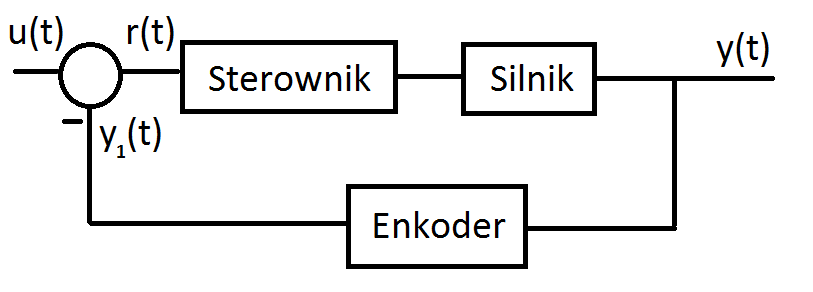
\includegraphics[scale=0.45]{imgs/sterowanie.png}
 	\caption[Schemat pętli sterowania silnikami.]{\small{Schemat przedstawia koncepcję pętli sterowania silnikami napędowymi. Ujemne sprzężenie zwrotne realizowane jest przy wykorzystaniu enkodera impulsowego. Sygnały: $u(t)$ - wartość zadana, $r(t)$ - uchyb, $y(t)$ wyjście układu.}}
	\label{schem_ster}
    \end{center}
  \end{figure}  
  
\namedsection{Programowanie}
Programowanie Atmegi odbywa się przy wykorzystaniu programatora, czyli specjalnego układu elektronicznego służącego do sprzęgnięcia komputera z mikrokontrolerem zgodnie z rysunkiem \ref{schem_ster}. Urządzenie realizuje komunikację jednostronną, tzn. przesyła jedynie program do wewnętrznej pamięci układu scalonego.  Programowanie odbywa się przy wykorzystaniu magistrali SPI, która ,,wybiera" układ docelowy przy pomocy linii SS (ang. \textit{Slave Select}) a następnie przesyła dane wykorzystując linie MISO, MOSI. Linia SCK służy do synchronizacji przebiegów szeregowych. Z racji tego, że programowany jest tylko jeden, aktualnie podłączony układ, linię SS można zaniechać.

  \begin{figure}[H]
    \begin{center}
      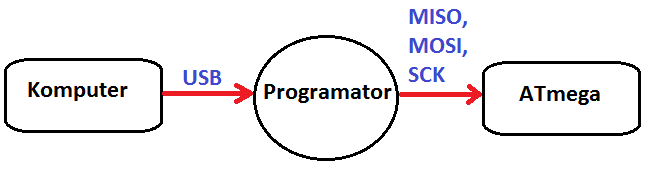
\includegraphics[scale=0.7]{imgs/schemat_prog.png}
 	\caption[Podłączenie programatora.]{\small{Graf przedstawiający idee pracy programatora. ATmega przyjmuje dane posługując się następującymi pinami : MISO (ang. \textit{Master Input Slave Output} - przyjmowanie danych), MOSI (ang. \textit{Master Output Slave Input} - nadawanie danych) oraz SCK - zegar taktujący. Wymienione piny pozwalają na realizacje transmisji typu SPI (ang. \textit{Serial Peripheral Interface}) pozwalającej na komunikacje jednostki centralnej z układami peryferyjnymi.}}
	\label{schem_ster}
    \end{center}
  \end{figure}  
  
\namedsection{Prędkość obrotowa}
Prędkość obrotowa, a konkretniej częstotliwość obrotu, jest odczytywana przy wykorzystaniu enkoderów impulsowych. W jego skład wchodzi niewielkie koło, na którego obwodzie są obsadzone magnesy. Urządzenie pomiarowe jest układem scalonym umieszczonym nieco ponad obracającym się kołem. Czujnik działa w oparciu o efekt Halla i na wyjściu generuje falę prostokątną o częstotliwości około 355 impulsów na jeden pełny obrót wału. Częstotliwość obrotu silnika jest obliczana na podstawie częstotliwości wspomnianej fali prostokątnej. Pomiar zaimplementowany jest na mikrokontrolerze Atmega48. Jego ogólna koncepcja przedstawiona została na rysunku \ref{predkosc}.  

  \begin{figure}[H]
    \begin{center}
      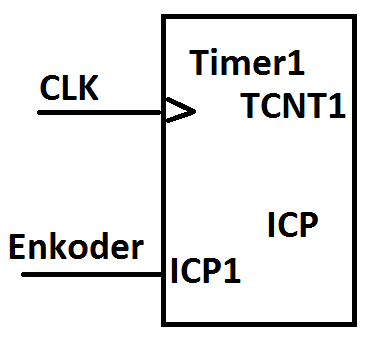
\includegraphics[scale=0.7]{imgs/predkosc.png}
 	\caption[Pomiar częstotliwości obrotu silnika.]{\small{Ilustracja przedstawia ideę pomiaru częstotliwości obrotu silników napędowych. Timer1 jest wewnętrznym, sprzętowym licznikiem mikrokontrolera. Na wyprowadzeniu pinu Atmegi ICP1 podłączony jest enkoder. Licznik taktowany jest wewnętrznym zegarem. W momencie wystąpienia zbocza narastającego na pinie ICP1 aktualna wartość licznika, przechowywana w rejestrze TCNT1 zapisywana jest do rejestru ICP. Znając szybkość taktowania licznika oraz ilość zliczonych impulsów pomiędzy dwoma narastającymi zboczami enkodera możliwe jest obliczenie częstotliwości obrotu wału silnika.}}
	\label{predkosc}
    \end{center}
  \end{figure}  
